\documentclass{beamer}

\usepackage[utf8]{inputenc}%uso utf8 invece di utf8x per poter mettere gli accenti nel titolo del pdf. Questo mi crea problemi con i °
\usepackage{default}
\usepackage[italian]{babel}
\usepackage{graphicx}
\usepackage[version=3]{mhchem} % Formula subscripts using \ce{}
\usepackage{multicol}
\renewcommand{\thefootnote}{}%elimina il numerino della nota a piè di pagina
\renewcommand\footnoterule{}%elimina la riga prima della nota a piè di pagina

\usetheme{Warsaw}        % layout complessivo. 
\useinnertheme{default} % layout interno.
\useoutertheme{default} % layout esterno.
\usecolortheme{wolverine} % schema di colori.
\usefonttheme{default}  % schema dei font.

\hypersetup{pdfauthor={Ilario Gelmetti},pdfsubject={Polimeri coniugati per applicazioni fotovoltaiche},pdfkeywords={polimeri coniugati, fotovoltaico, politiofene, carbazolo, tiofene, policarbazolo, fluorene, polifluorene, fenilenevinilene, perilene bisimmide, fullerene, polimeri a blocchi, rod-rod, rod-coil},pdftitle={Polimeri coniugati per applicazioni fotovoltaiche}} %metadati nel pdf


\setbeamertemplate{navigation symbols}{} %per eliminare i bottoni della barra di navigazione in basso a destra
\AtBeginSection[]{\frame{\tableofcontents[current,hideothersubsections]}} %indice all'inizio di ogni section, mostra solo le sottosezioni di quella sezione
\newcommand{\nsub}[1]{\subsection{#1}\begin{frame}\frametitle{#1}} %scorciatoia per nuova diapo con nuova subsection


\title[Polimeri coniugati per applicazioni fotovoltaiche]{Polimeri coniugati per applicazioni fotovoltaiche}
\subtitle{Esame di Complementi di Chimica Macromolecolare.}
\author{Ilario Gelmetti}
\institute{Scuola Normale Superiore di Pisa.\\Professore Giancarlo Galli.}
\date{12 ottobre 2011}
\logo{
\includegraphics[width=0.07\paperwidth]{img/snslogo.png}}

\begin{document}
\begin{frame}
  \titlepage
\end{frame}

\section{Introduzione}
\diapo{La chimica del silicio}
Il silicio come ``{\bf traghettatore}'': 
$$\ce{R ->[?] P}$$
$$\ce{R ->C[+Si] I ->[-\ce{Si}] P}$$
\pause
I {\bf legami del silicio}:
\begin{itemize}
 \item {\bf facile rottura} eterolitica da parte di reagenti ionici, {\bf ossigeno e alogeni};
 \item se {\bf legato al carbonio} può essere considerato un {\bf super-protone};
 \item se {\bf legato all'ossigeno} può essere considerato un {\bf protone indebolito}.
\end{itemize}
\end{frame}


%%%%%%%%%%%%%%%%%%%%%%%%%%%%%%%%%%%%%%%%%%%%%%%%%%%%%%%%%%%%%%%%%%%%
\logo{}

\begin{frame}
\frametitle{La chimica del silicio}
\begin{block}{Effetto $\beta$: ($\sigma$--p)$_\pi$}
\begin{figure}{\centering{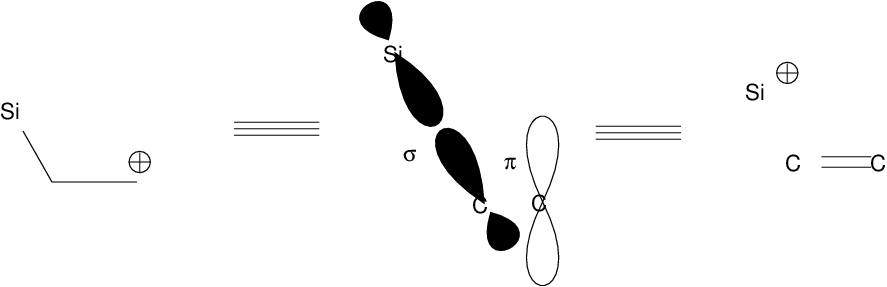
\includegraphics[width=0.7\textwidth]{img/intro/b-effect.png}}}\end{figure}
\end{block}
\pause
\begin{block}{$\alpha$ anioni: ($\sigma$*--p)$_\pi$}
\begin{figure}{\centering{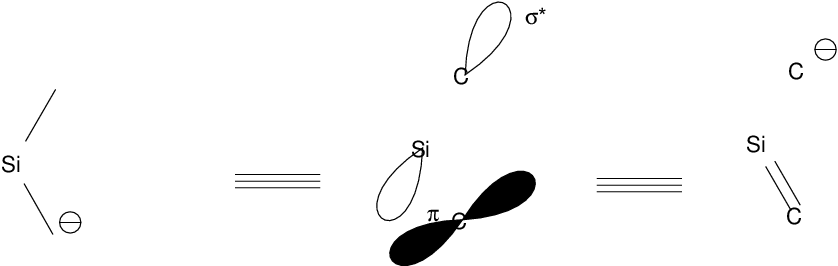
\includegraphics[width=0.7\textwidth]{img/intro/a-anions.png}}}\end{figure}
\end{block}
\end{frame}

\logo{
\includegraphics[width=0.07\paperwidth]{img/snslogo.png}}

%%%%%%%%%%%%%%%%%%%%%%%%%%%%%%%%%%%%%%%%%%%%%%%%%%%%%%%%%%%%%%%%%%%%

\diapo{Schema generale delle reazioni di interesse}
\begin{figure}{\centering{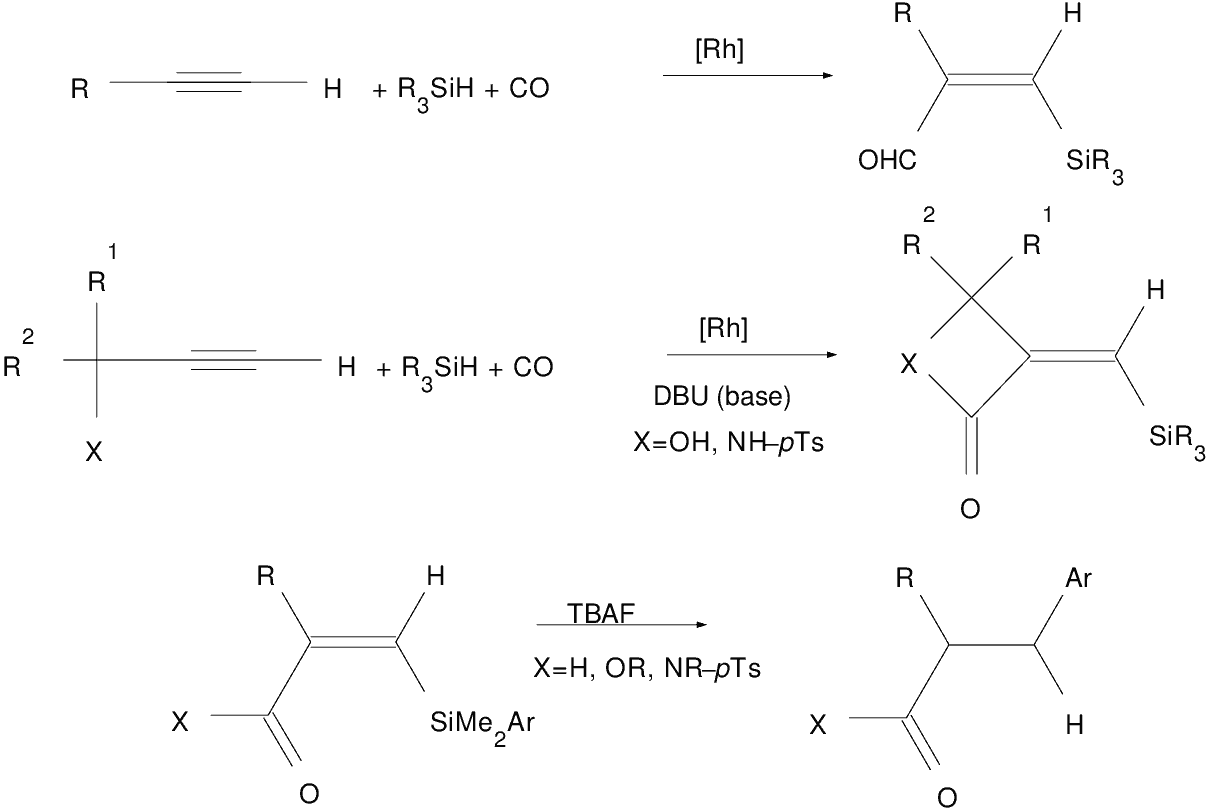
\includegraphics[width=0.8\textwidth]{img/intro/generale.png}}}\end{figure}


\end{frame}

\subsection{Prodotti ottenibili da $\beta$-silil alchenali}\begin{frame}\frametitle{Prodotti ottenibili da $\beta$-silil alchenali}
I $\beta$-sililalchenali ottenuti possono poi essere trasformati sfruttando la {\bf reattività sia di un carbonile $\alpha , \beta $ insaturo sia di un vinil silano}.
\begin{figure}{\centering{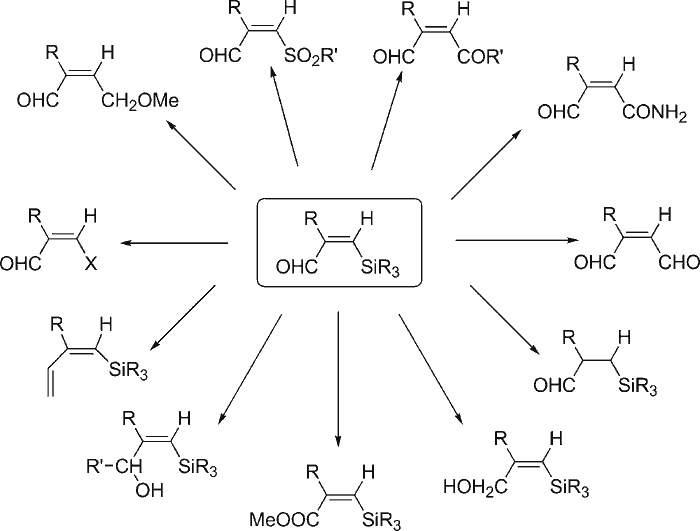
\includegraphics[width=0.6\textwidth]{img/intro/altri_prodotti_ottenibili.png}}}\end{figure}


\end{frame}


%%%%%%%%%%%%%%%%%%%%%%%%%%%%%%%%%%%%%%%%%%%%%%%%%%%%%%%%%%%%%%%%%%%%




\section{Principali polimeri coniugati donatori}
\nsub{Basati su $p$-fenilene vinilene}
\footnotesize{Via Wessling, la via storica:}
\begin{figure}{\centering{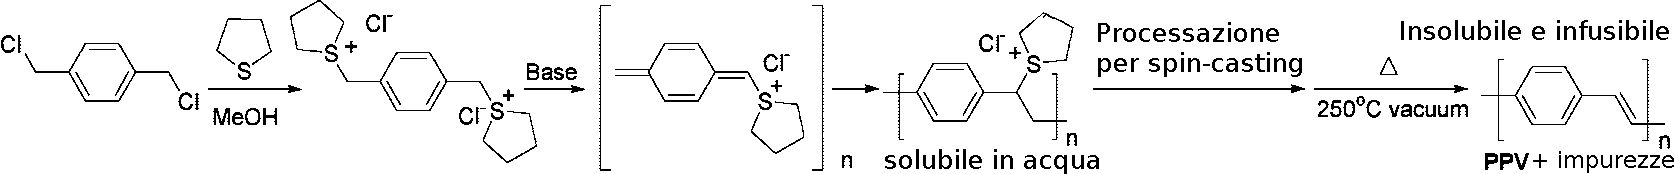
\includegraphics[width=1\textwidth]{img/ppv2.png}}}\end{figure}
\footnotesize{Via Glich (i gruppi alcossi abbassano il LUMO):}
\begin{figure}{\centering{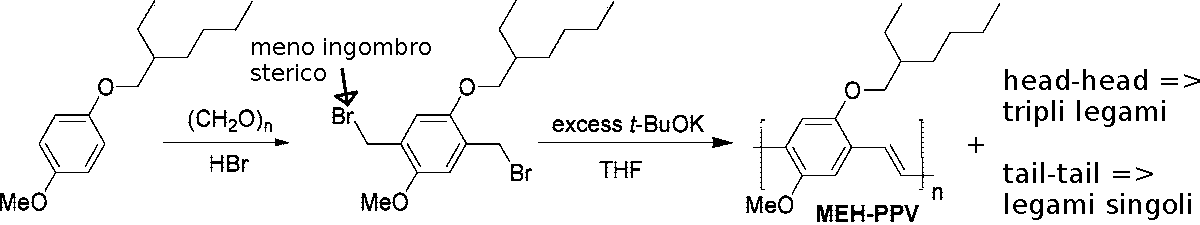
\includegraphics[width=0.85\textwidth]{img/ppv-meh.png}}}\end{figure}
\footnotesize{Via Wittig-Horner per avere maggiore regioregolarità:}
\begin{figure}{\centering{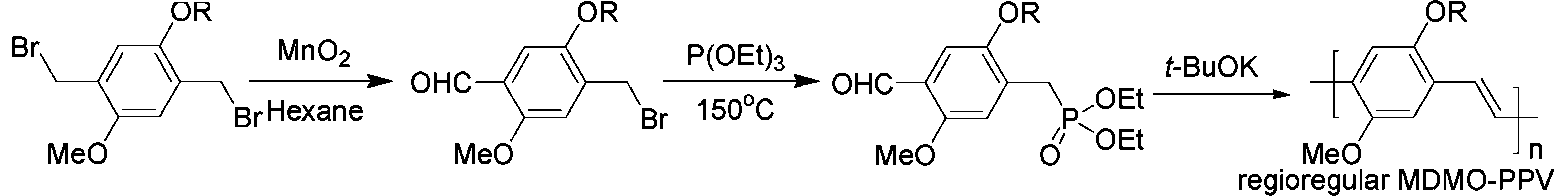
\includegraphics[width=0.95\textwidth]{img/ppv-wittig.png}}}\end{figure}
\end{frame}
%%%%%%%%%%%%%%%%%%%%%%%%%%%%%%%%%%%%%%%%%%%%%%%%%%%%%%%%%%%%%%%%%%%%%%%%%%%%%%%%%%%%%%%%%%%%%%%%%%%%%%%%%%%%%%%%%%%%%%%%%%%%%%
\subsubsection{Variazioni sulla struttura}\begin{frame}\frametitle{Basati su $p$-fenilene vinilene}\framesubtitle{Variazioni sulla struttura}
 \begin{columns}
\column{0.3\linewidth} 
{Aumentato assorbimento e trasporto lacune. Diminuito \emph{band~gap}.}
\begin{figure}{\centering{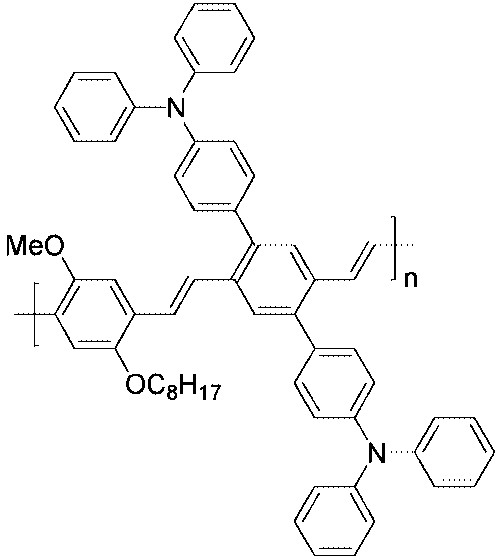
\includegraphics[width=1\textwidth]{img/ppv-ammina.png}}}\end{figure}
\column{0.7\linewidth}
{Tiofene elettronricco e poco aromatico, \emph{band gap} minore. Polimerizzazione ossidativa con \ce{FeCl3}.}
\vspace{-15pt}\begin{figure}{\centering{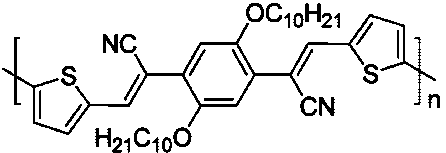
\includegraphics[width=0.5\textwidth]{img/ppv-cn-tio.png}}}\end{figure}
{Più linearità quindi migliore cristallizzazione.}
\begin{figure}{\centering{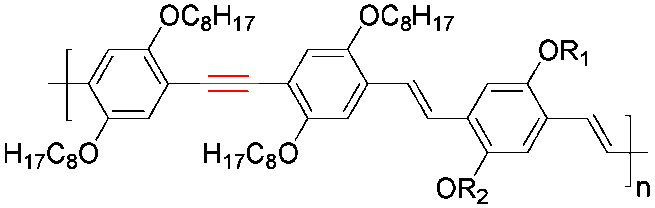
\includegraphics[width=0.8\textwidth]{img/ppv-ino.png}}}\end{figure}

\end{columns}
\end{frame}
\nsub{Basati su fluorene}
Vantaggi dei polimeri a base di 9,9-dialchilfluorene:
\begin{itemize}
 \item ottima conduzione di lacune: $I_{short-circuit}$ maggiori;
 \item possibile ottenere film;
 \item stabilità alle ossidazioni: HOMO basso, $V_{open-circuit}$ maggiori;
\end{itemize}
Svantaggio: \emph{band gap} troppo grande (scarso assorbimento).

Per diminuire il \emph{band gap} si polimerizza un dimero fluorene-composto elettron-ricco (bitiofene o pentacene o antraditiofene) via Suzuki:
\begin{figure}{\centering{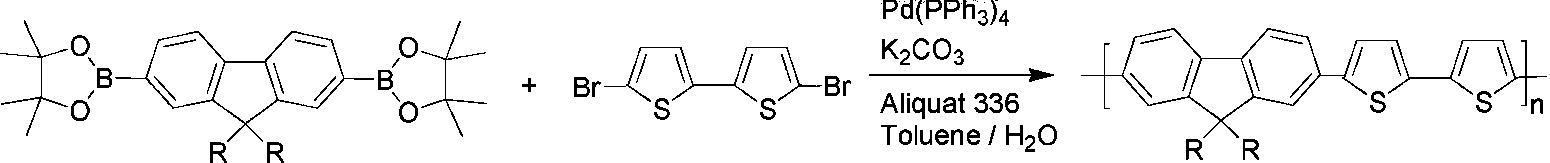
\includegraphics[width=1\textwidth]{img/fluo-tio.png}}}\end{figure}

\end{frame}
\subsubsection{Utilizzo di gruppi ausiliari}\begin{frame}\frametitle{Basati su fluorene}\framesubtitle{Utilizzo di gruppi ausiliari}
\begin{columns}\column{0.6\linewidth}Oppure si può utilizzare un monomero contenente unità elettron-donatori (tiofene) e elettron-accettori (2,1,3-benzotiadiazolo) per ottenere una nuova banda di assorbimento a $\lambda$ grandi per il trasferimento di carica.
\column{0.4\linewidth}\vspace{-35pt}\begin{figure}{\centering{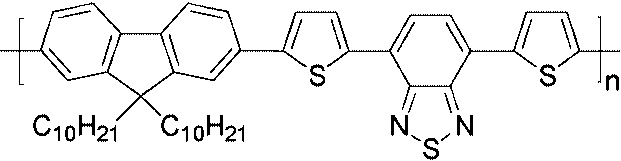
\includegraphics[width=1\textwidth]{img/fluo-tiaza.png}}}\end{figure}
\end{columns}\vspace{10pt}
\begin{columns}\column{0.5\linewidth}\begin{figure}{\centering{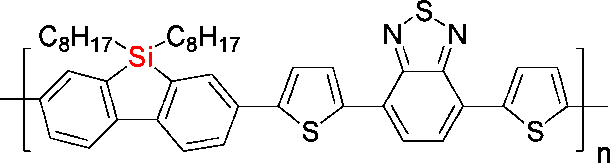
\includegraphics[width=1\textwidth]{img/fluo-si.png}}}\end{figure}
\column{0.6\linewidth}Sostituendo il C9 con Si si ottiene una diminuzione del \emph{band gap} (più assorbimento; silolo ha $\Delta E_{HOMO-LUMO}$ piccolo), un abbassamento del HOMO ($V_{open-circuit}$ maggiore) e altissima mobilità di lacune.
\end{columns}

\end{frame}

%%%%%%%%%%%%%%%%%%%%%%%%%%%%%%%%%%%%%%%%%%%%%%%%%%%%%%%%%%%%%%%%%%%%%%%%%%%%%%%%%%%%%%%%%%%%%%%%%%%%%%%%%%%%%%%%%%%%%%%%%%%%%%
\logo{}
\nsub{Basati su carbazolo}
L'azoto 
rende aromatico e elettron-donatore il carbazolo. Forma cationi stabili ed ha una buona mobilità di lacune.

\vspace{-6pt}\begin{figure}{\centering{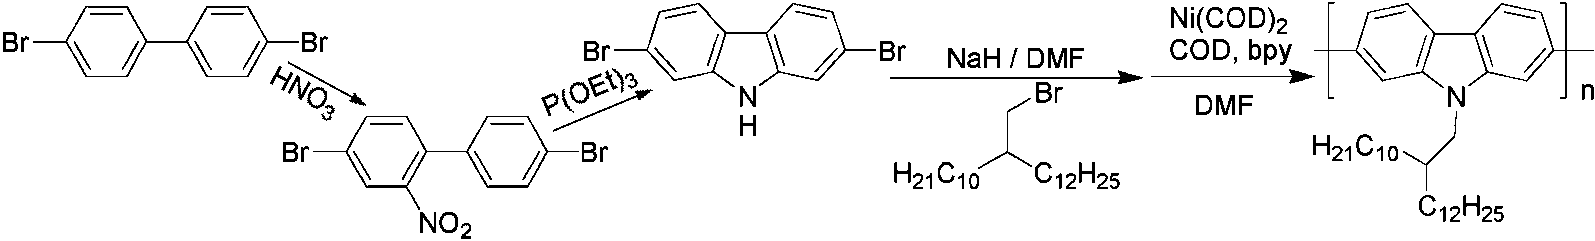
\includegraphics[width=1\textwidth]{img/carbaz-sint.png}}}\end{figure}
\vspace{-12pt}Unità elettron-attrattrici incorporate per abbassare il \emph{band gap}.\\ Sistemi indolocarbazolo più donatori e più cristallini (più conduzione e più assorbimento).
\vspace{-10pt}\begin{columns}\column{0.4\linewidth}\begin{figure}{\centering{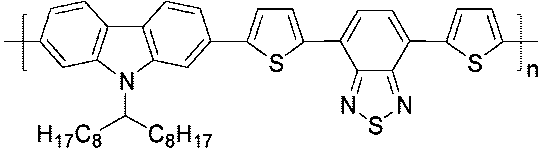
\includegraphics[width=1\textwidth]{img/carbaz-tio.png}}}\end{figure}\column{0.6\linewidth}\begin{figure}{\centering{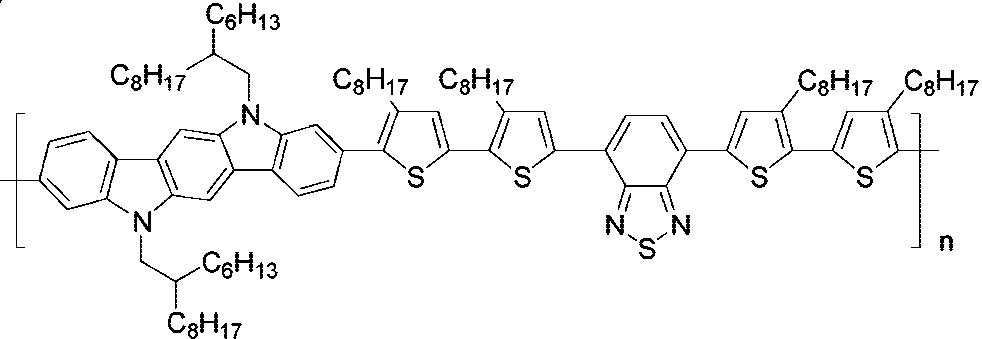
\includegraphics[width=1\textwidth]{img/carbaz-indolo.png}}}\end{figure}\end{columns}
\end{frame}
\logo{
\includegraphics[width=0.07\paperwidth]{img/snslogo.png}}

%%%%%%%%%%%%%%%%%%%%%%%%%%%%%%%%%%%%%%%%%%%%%%%%%%%%%%%%%%%%%%%%%%%%%%%%%%%%%%%%%%%%%%%%%%%%%%%%%%%%%%%%%%%%%%%%%%%%%%%%%%%%%%
\nsub{Basati su tiofene}
Molto impiegato è il poli(3-esiltiofene) regioregolare \emph{head-tail}, 
\begin{itemize}
 \item una catena laterale più corta non rende solubile il polimero, più lunga favorisce la separazione di fase nella cella solare;
 \item regioregolarità per avere planarità (coniugazione) e cristallinità (conduzione intercatena e assorbimento);
 \item cristallinità se eccessiva provoca separazione di fase durante la fase di \emph{annealing} (perciò si inseriscono difetti nella catena tramite un comonomero); se troppo scarsa (per catene troppo corte) si ha difficile conduzione intercatena e minore assorbimento.
\end{itemize}\end{frame}
\subsubsection{Ciclo catalitico della polimerizzazione}\begin{frame}\frametitle{Basati su tiofene}\framesubtitle{Ciclo catalitico della polimerizzazione}
\small{La sintesi via metatesi Grignard e coupling di Kumada-Corriu porta a una polimerizzazione vivente con bassa polidispersità. }
\begin{figure}{\centering{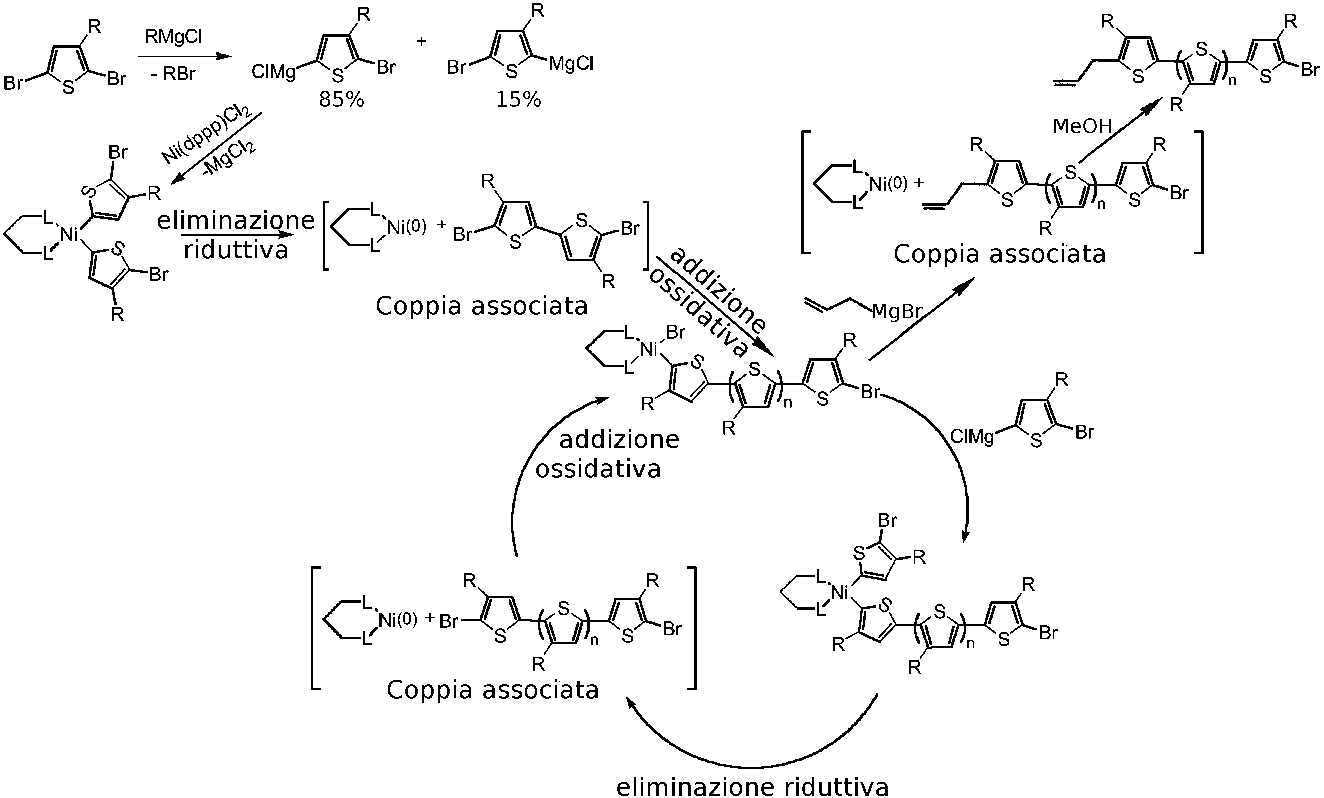
\includegraphics[width=0.85\textwidth]{img/pol-grim-polimerizz3.png}}}\end{figure}
\end{frame}





\subsubsection{Politiofene con catene laterali coniugate}\begin{frame}\frametitle{Basati su tiofene}\framesubtitle{Politiofene con catene laterali coniugate}
Gruppi laterali coniugati per aumentare l'assorbimento.
\begin{columns}\column{0.6\linewidth}Inoltre HOMO abbassato: $V_{open-circuit}$ maggiore senza perdita di assorbimento.
\column{0.4\linewidth}\vspace{-20pt}\begin{figure}{\centering{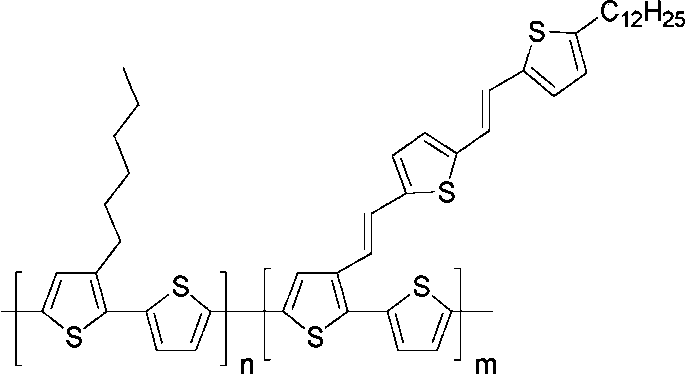
\includegraphics[width=1\textwidth]{img/p3ht-conj-tio.png}}}\end{figure}
\end{columns}\vspace{-20pt}
\begin{columns}\column{0.3\linewidth}\begin{figure}{\centering{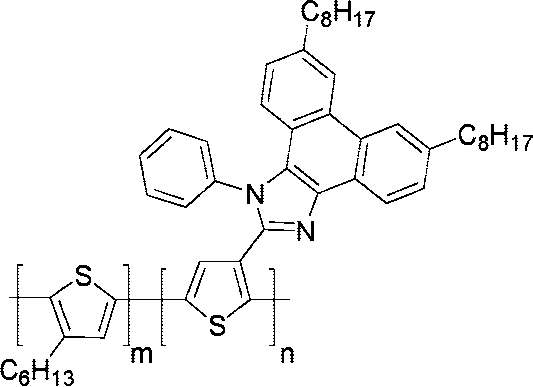
\includegraphics[width=1\textwidth]{img/p3ht-conj-accept.png}}}\end{figure}
\column{0.7\linewidth}Inoltre accettore intermedio di $e^-$: facilita il trasferimento al materiale accetore.
\end{columns}\vspace{5pt}
Dei politiofeni reticolati con ponti coniugati per aumentare la mobilità di lacune hanno mostrato peggioramento delle caratteristiche a causa della deformazione indotta.
\end{frame}




\subsubsection{Politiofene con anelli fusi in 3,4}\begin{frame}\frametitle{Basati su tiofene}\framesubtitle{Politiofene con anelli fusi in 3,4}
\begin{columns}
\column{0.25\linewidth}
\begin{figure}{\centering{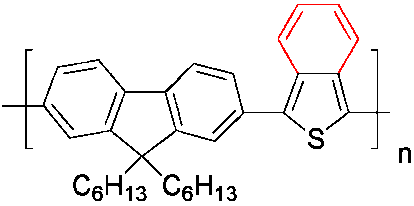
\includegraphics[width=1.1\textwidth]{img/tio-fus-benz-fluo.png}}}\end{figure}
\column{0.75\linewidth}Fondendo un anello benzenico sull'anello tiofenico si aumenta il peso della forma chinonica e si ottengono (per polimerizzazione elettrochimica, termica o ossidativa con \ce{FeCl3}) polimeri con \emph{band gap} e peso molecolare troppo bassi e con scarsa stabilità chimica. Può essere utilizzato in con fluorene per abbassarne il \emph{band gap}.
\end{columns}
\vspace{10pt}\begin{columns}
\column{0.6\linewidth}Anche il tieno[3,4-$b$]tiofene può servire per abbassare il \emph{band gap} a seconda del contenuto nel polimero. Nella figura la catena perfluorurata stabilizza l'anello elettronricco.
\column{0.3\linewidth}\vspace{-20pt}\begin{figure}{\centering{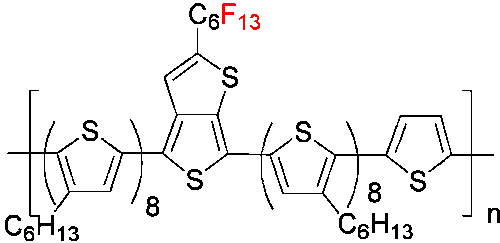
\includegraphics[width=1\textwidth]{img/tio-fus-tio.png}}}\end{figure}
\end{columns}
\end{frame}


\subsubsection{Politiofene con anelli fusi in 2,3}\begin{frame}\frametitle{Basati su tiofene}\framesubtitle{Politiofene con anelli fusi in 2,3}
Un carbonio a ponte aumenta la planarità e diminuisce il \emph{band gap}.\vspace{10pt}\begin{columns}\column{0.5\linewidth}
Il gruppo elettron-attrattore diminuisce il \emph{band gap} ed aumenta le interazioni intermolecolari. Il secondo blocco assorbe a frequenze diverse. 
\column{0.5\linewidth}
\begin{figure}{\centering{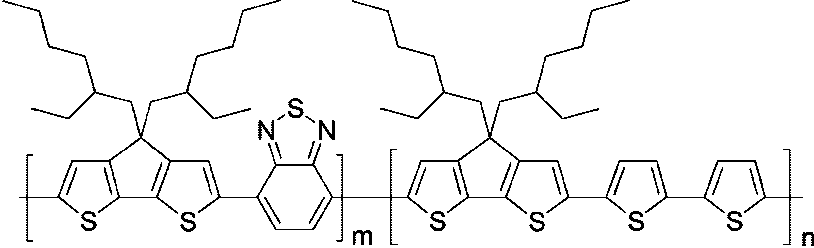
\includegraphics[width=1\textwidth]{img/tio-fus-penta.png}}}\end{figure}
\end{columns}
\begin{columns}\column{0.3\linewidth}\begin{figure}{\centering{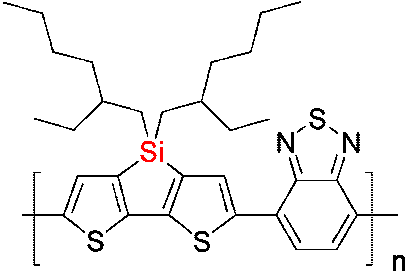
\includegraphics[width=1\textwidth]{img/tio-fus-si.png}}}\end{figure}
\column{0.6\linewidth}Come nel fluorene, usare un Si come ponte permette di avere mobilità elettroniche 3 volte maggiori, HOMO più basso e assorbimento fino a 800nm (\emph{band gap} minore).
\end{columns}
\end{frame}



\subsubsection{Politiofene con vinileni o etinileni}\begin{frame}\frametitle{Basati su tiofene}\framesubtitle{Politiofene con vinileni o etinileni}
\begin{columns}
\column{0.3\linewidth}
\vspace{-10pt}
\begin{figure}{\centering{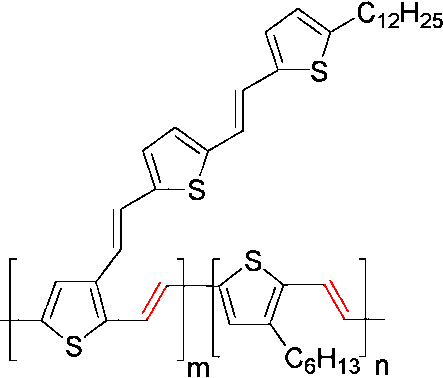
\includegraphics[width=1\textwidth]{img/tio-vinilene.png}}}\end{figure}
\column{0.7\linewidth}
Inserendo unità vinilene si riduce l'aromaticità, aumenta la planarità, la coniugazione, si assorbe molto più spettro. Per aggirare problemi di difficile processabilità è possibile rendere coniugato il polimero \emph{in situ}. 
\end{columns}
\begin{columns}
\column{0.6\linewidth}Il triplo legame da rigidità ed aumenta la coniugazione. Nella figura un gruppo donatore ed uno accettore danno un polimero con basso \emph{band gap}.
\column{0.3\linewidth}\begin{figure}{\centering{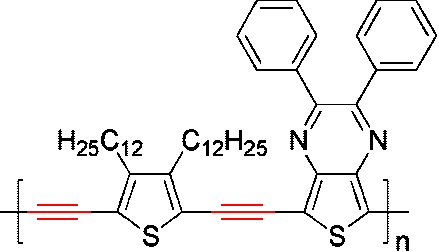
\includegraphics[width=1\textwidth]{img/tio-ino.png}}}\end{figure}
\end{columns}
\end{frame}





%%%%%%%%%%%%%%%%%%%%%%%%%%%%%%%%%%%%%%%%%%%%%%%%%%%%%%%%%%%%%%%%%%%%%%%%%%%%%%%%%%%%%%%%%%%%%%%%%%%%%%%%%%%%%%%%%%%%%%%%%%%%%%

\nsub{Esempi di altri polimeri donatori}
\begin{columns}
\column{0.6\linewidth}Una politriarilammina non è coniugata lungo la catena a causa dell'azoto e non è planare. Ciò nonostante, grazie alla coppia con un gruppo elettron-attrattore, può avere un basso \emph{band gap}.
\column{0.4\linewidth}
\begin{figure}{\centering{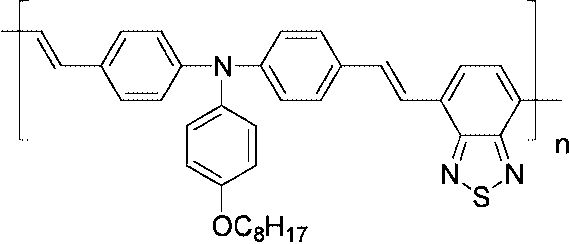
\includegraphics[width=1\textwidth]{img/ammina.png}}}\end{figure}
\end{columns}
\vspace{10pt}
\begin{columns}
\column{0.5\linewidth}\vspace{-10pt}\begin{figure}{\centering{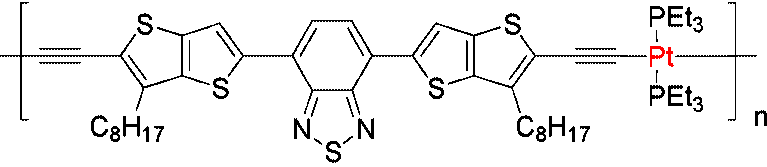
\includegraphics[width=1\textwidth]{img/platino.png}}}\end{figure}
\column{0.5\linewidth}Un atomo di platino permette un efficiente \emph{intersystem crossing} formando stati eccitati di tripletto ossia eccitoni con tempi di vita più lunghi e minore ricombinazione di cariche.
\end{columns}
\end{frame}


\section{Copolimeri a blocchi accettore-donatore}% - punto di vista accettore}
\nsub{I polimeri elettron-accettori}\footnotetext{\tiny{\cite{5}DOI: 10.1021/ma102566u}}
Il materiale elettron-accettore (di tipo~n) più usato è fullerene funzionalizzato PCBM (è solubile ed ha ottime proprietà di elettron-accettore e trasportatore di elettroni) oppure nanoparticelle inorganiche.

A causa della sua simmetria il fullerene ha assorbimento solo ad alte energie.

L'alternativa di impiegare polimeri coniugati elettron-accettori porta a grossi problemi di smescolamento.
\begin{columns}\column{0.5\linewidth}
\begin{figure}{\centering{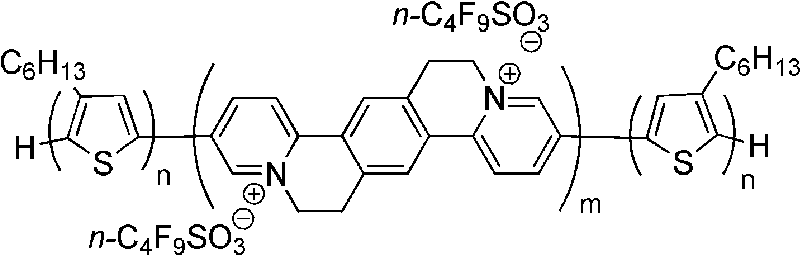
\includegraphics[width=1\textwidth]{img/dba-piridin-tio.png}}}\end{figure}\column{0.5\linewidth}
Esempio di polimero a blocchi donatore-accettore-donatore.

\end{columns}
\end{frame}



% %%%%%%%%%%%%%%%%%%%%%%%%%%%%%%%%%%%%%%%%%%%%%%%%%%%%%%%%%%%%%%%%%%%%%%%%%%%%%%%%%%%%%%%%%%%%%%%%%%%%%%%%%%%%%%%%%%%%%%%%%%%%%%

\nsub{Basati su fullerene}
Per evitare lo smescolamento del fullerene si può:
\begin{enumerate}
 \item fullerene legato alle catene laterali del polimero donatore (polimeri ``doppio cavo'') ma si ha ricombinazione di cariche;
 \item copolimero a blocchi donatore-(blocco con fullereni in catena laterale o al termine) non troppo funzionalizzato per garantire la percolazione ed evitare la reticolazione;
 \item copolimero a blocchi donatore-(polimero con gruppi leganti di fullereni);
 \item un copolimero a blocchi come compatibilizzante.
\end{enumerate}
Se la catena con i fullereni è non coniugata fungerà da isolante. Al contrario se è coniugata si ha un migliore trasferimento\\(\emph{quenching} di fotoluminescenza).
 \end{frame}

\subsubsection{Esempi di accettori con fullereni}\begin{frame}\frametitle{Basati su fullerene}\framesubtitle{Esempi di accettori con fullereni}
\begin{figure}{\centering{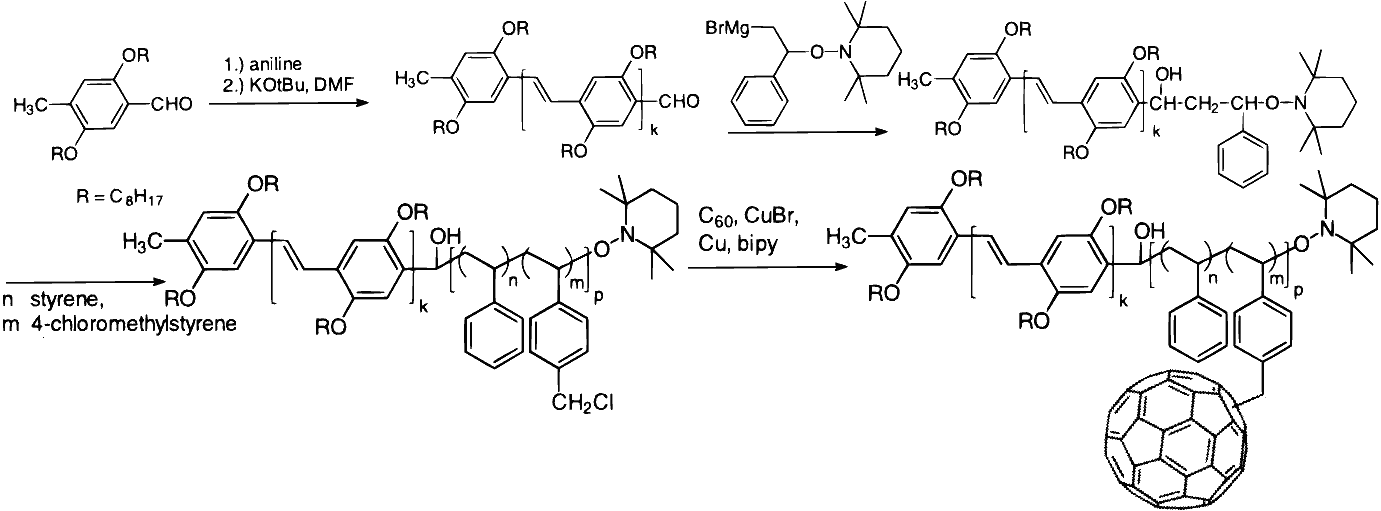
\includegraphics[width=0.8\textwidth]{img/dba-fu-ps-ppv.png}}}\end{figure}\vspace{-30pt}{\tiny{\cite{2}DOI: 10.1021/ja000160a}} 
\begin{figure}{{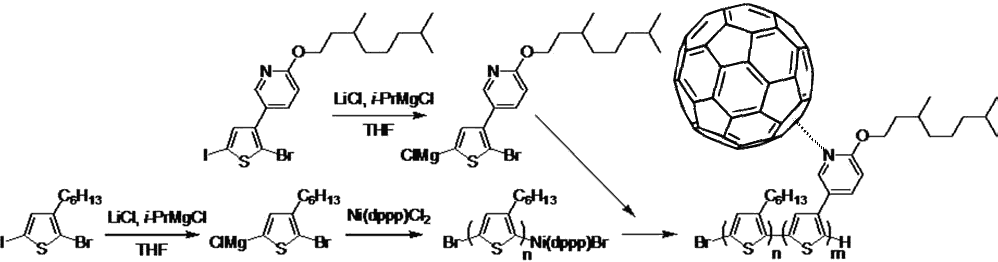
\includegraphics[width=0.8\textwidth]{img/dba-fu-tio-tioleg.png}}}\end{figure}\tiny{\cite{3}DOI: 10.1002/pola.24689} 
\end{frame}


\subsubsection{Polimeri a blocchi come compatibilizzanti}\begin{frame}\frametitle{Basati su fullerene}\framesubtitle{Polimeri a blocchi come compatibilizzanti}
\footnotetext{\tiny{\cite{6}DOI: 10.1002/macp.201000080}}
\begin{columns} \column{0.5\linewidth}
I polimeri a blocchi possono essere utilizzati come compatibilizzanti di miscele polimero-fullerene o polimero donatore-polimero accettore. 
\column{0.5\linewidth}\vspace{-10pt}\begin{figure}{\centering{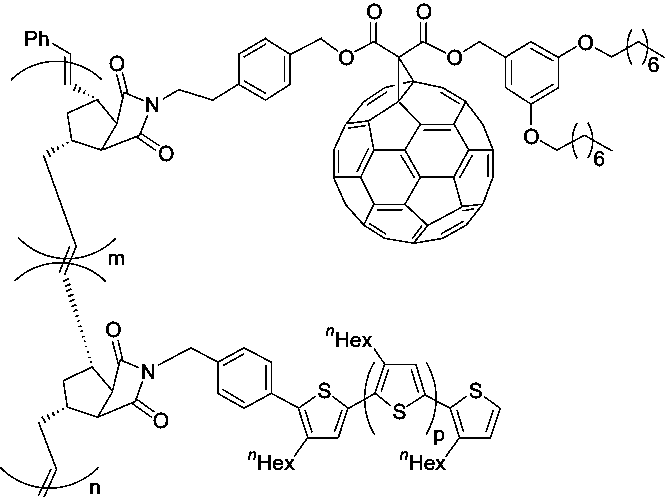
\includegraphics[width=0.9\textwidth]{img/dba-fu-tio.png}}}
\end{figure}\tiny{\cite{9}DOI: 10.1002/adma.200501787}
\end{columns}
\begin{figure}{{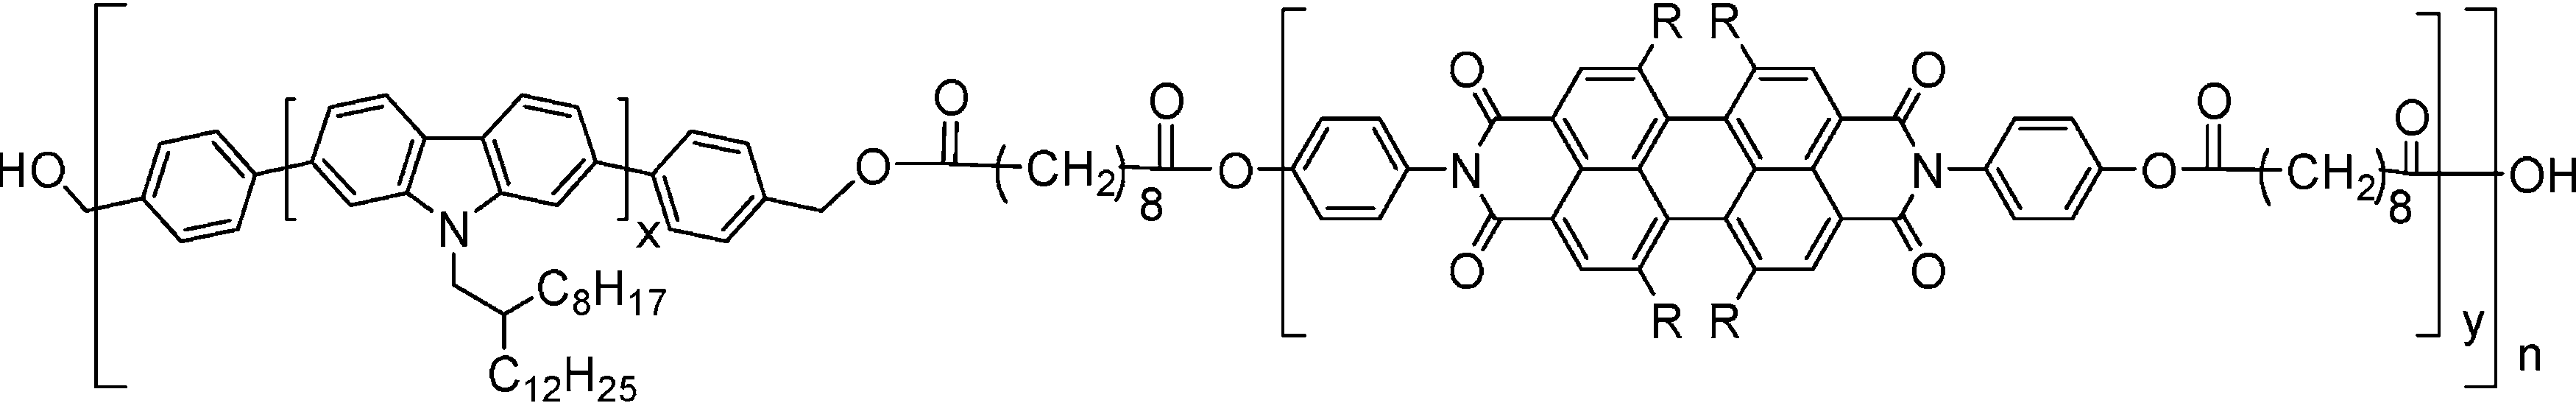
\includegraphics[width=0.9\textwidth]{img/dba-spacer.png}}}\end{figure}
\end{frame}

% %%%%%%%%%%%%%%%%%%%%%%%%%%%%%%%%%%%%%%%%%%%%%%%%%%%%%%%%%%%%%%%%%%%%%%%%%%%%%%%%%%%%%%%%%%%%%%%%%%%%%%%%%%%%%%%%%%%%%%%%%%%%%%
\nsub{Basati su perilene bisimmide}
\small{La eccessiva cristallizzazione del perilene bisimmide può essere limitata impiegandolo in un polimero a blocchi. La sintesi NMRP in figura usa come donatore tetrafenilbenzidina (HOMO e LUMO adatti, mobilità di lacune maggiore della trifenilammina (ma peggior macroiniziatore), i sostituenti donatori metossi aumentano la solubilità ed innalzano il HOMO).}
\begin{figure}{\centering{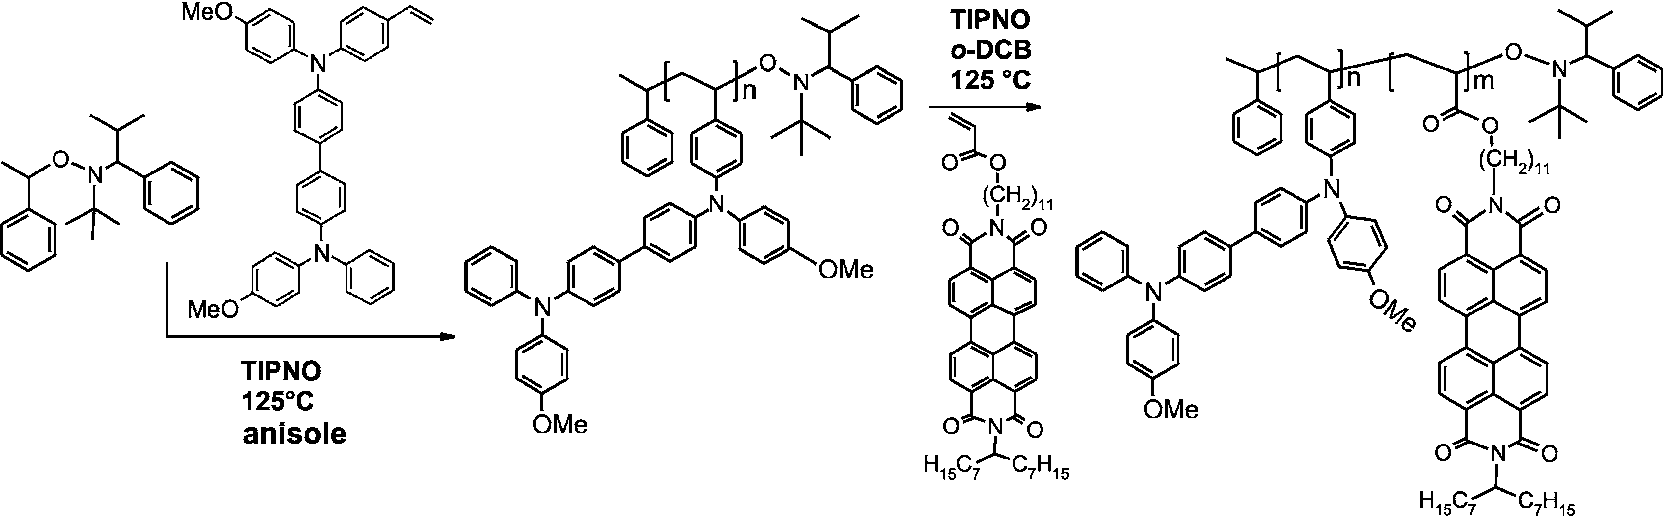
\includegraphics[width=1\textwidth]{img/dba-pbi-vtpa.png}}}
\end{figure}\vspace{-10pt}{\tiny{\cite{10}DOI: 10.1007/12\_2009\_34}}
\end{frame}

% %%%%%%%%%%%%%%%%%%%%%%%%%%%%%%%%%%%%%%%%%%%%%%%%%%%%%%%%%%%%%%%%%%%%%%%%%%%%%%%%%%%%%%%%%%%%%%%%%%%%%%%%%%%%%%%%%%%%%%%%%%%%%%

\nsub{Basati su $p$-fenilene vinilene}
Il carattere elettron-attrattore può essere proprio del monomero (come nel PBI o nel fullerene) oppure derivare da comonomeri o da modifiche strutturali su polimeri conduttori già visti.
\begin{figure}{{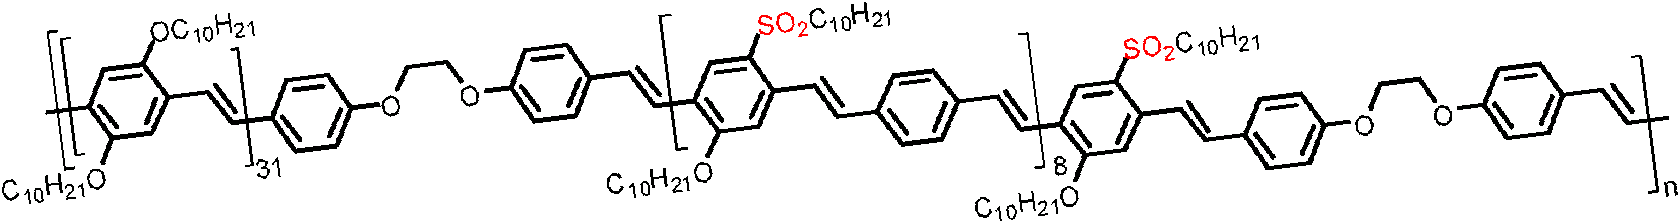
\includegraphics[width=0.9\textwidth]{img/dba-ppv-so2.png}}}\end{figure}\vspace{-10pt}{\tiny{\cite{7}DOI: 10.1063/1.2437100}}\\
CN abbassa HOMO e LUMO. In assenza di catene laterali sul blocco accettore Y è molto basso.
\begin{figure}{{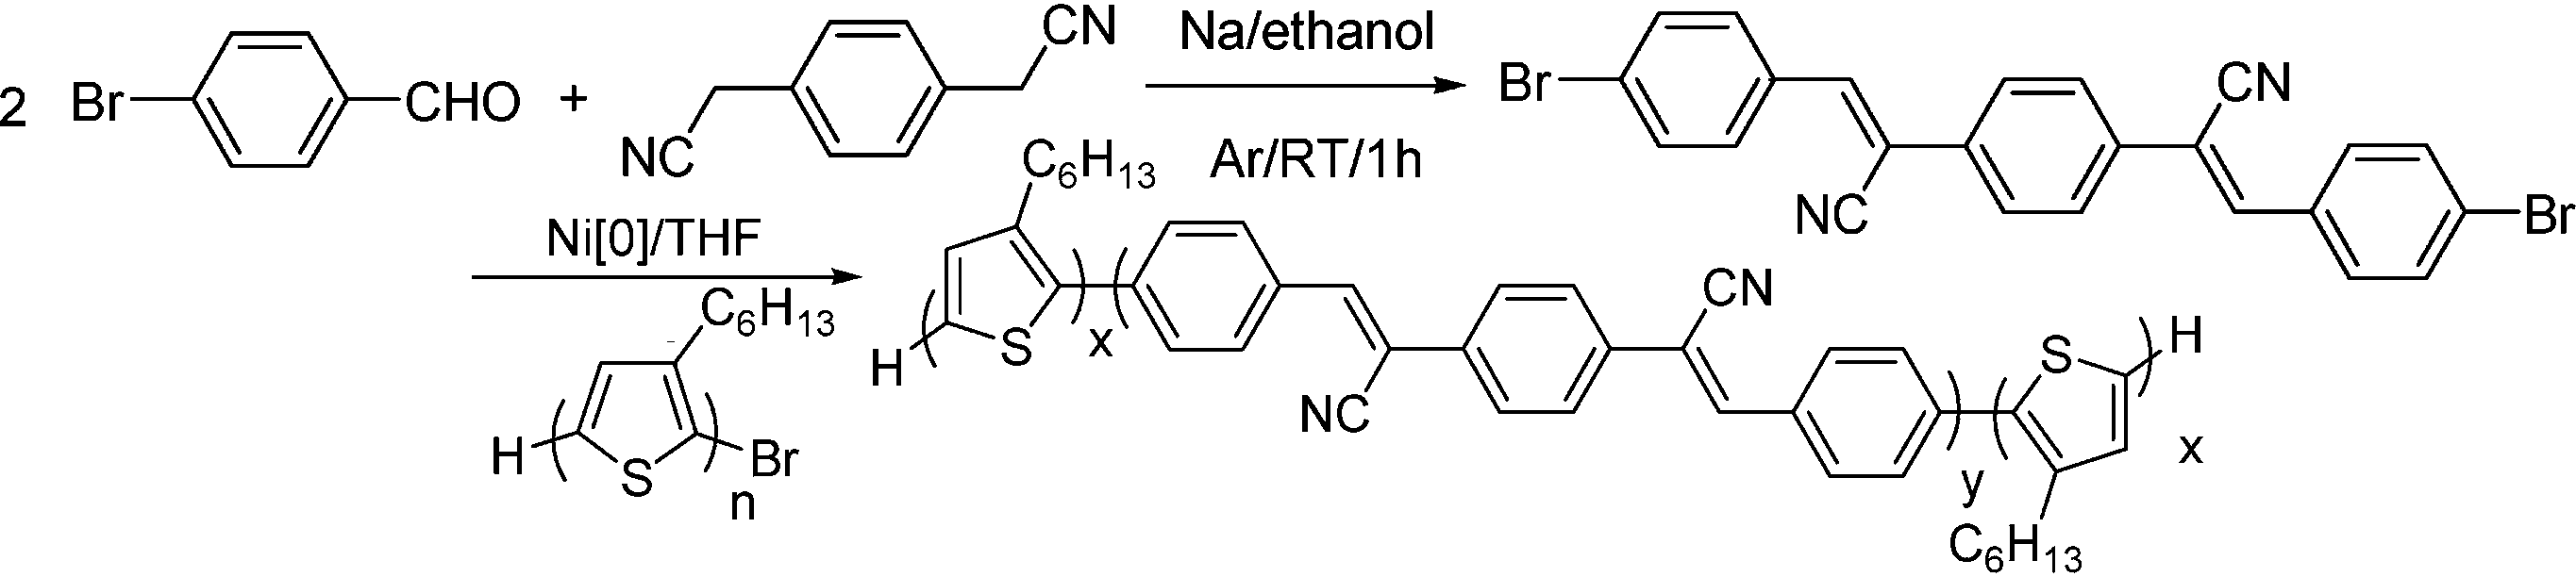
\includegraphics[width=0.8\textwidth]{img/dba-ppv-cn-tio.png}}}\end{figure}\vspace{-10pt}\tiny{\cite{8}DOI: 10.1021/ma060341i}

\end{frame}
% %%%%%%%%%%%%%%%%%%%%%%%%%%%%%%%%%%%%%%%%%%%%%%%%%%%%%%%%%%%%%%%%%%%%%%%%%%%%%%%%%%%%%%%%%%%%%%%%%%%%%%%%%%%%%%%%%%%%%%%%%%%%%%

\nsub{Basati su fluorene}In politiofene-$b$-polifluorene il polifluorene può essere utilizzato come elettron-accettore.
\begin{columns} \column{0.7\linewidth} Per facilitare l'auto-organizzazione si può rendere polare un blocco. In solventi di diversa polarità si avranno micelle o micelle inverse.
\column{0.25\linewidth}
\begin{figure}{{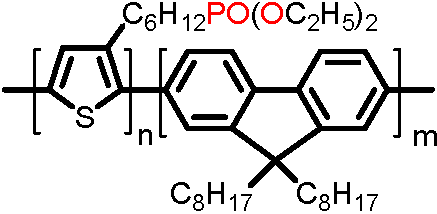
\includegraphics[width=1\textwidth]{img/dba-fluo-tiop.png}}}\\\vspace{-5pt}{\tiny{\cite{1}DOI: 10.1021/ar7002539}}\end{figure}
\column{0.05\linewidth}\end{columns}\vspace{10pt}
Copolimerizzando fluorene con benzotiadiazolo in modo \emph{random} utilizzando Suzuki si ottiene un miglior elettron-accettore. 
\begin{figure}{{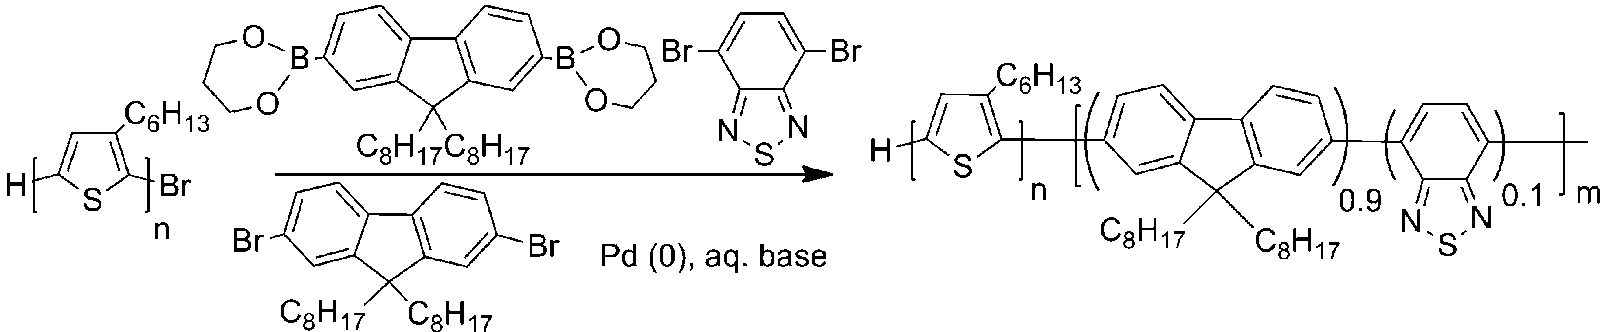
\includegraphics[width=0.8\textwidth]{img/dba-fluo-tio.png}}}\end{figure}\vspace{-5pt}{\tiny{\cite{4}DOI: 10.1021/ma102728z}}

\end{frame}


\setbeamertemplate{bibliography item}[text] %nella bibliografia in fondo ci mette i numeri invece del simbolo inutile del documento
\begin{frame}[plain,shrink]{%spappola la bibliografia per farla stare in una sola diapo

\begin{multicols}{2}
{\tiny{\bibliographystyle{abbrv}
\bibliography{Gelmetti-Sintesi_Polimeri_Coniugati.bib}
}}}\end{multicols}
\end{frame}
\end{document}
